%% Beamer Presentation using 16:9 aspect ratio (HDTV standard aspect ratio)
\documentclass[aspectratio=169]{beamer}

%% Metropolis or mtheme Theme
\usetheme{metropolis}

% Packages
\usepackage{fancyvrb}
\usepackage{graphicx}
\usepackage{listings}
\usepackage[]{hyperref, amsmath}
\usepackage{pgfplots}
\usepackage{appendixnumberbeamer}

% Provide an easy command for mono spaced font: \t{text}
\renewcommand{\t}[1]{\texttt{#1}}

% Provide an easy command for full screen graphics
\newcommand<>{\fullsizegraphic}[1]{
{
    \begin{frame}[plain]
        \begin{tikzpicture}[remember picture,overlay]
            \node[at=(current page.center)] {
                \includegraphics[width=\paperwidth]{#1}
            };
        \end{tikzpicture}
    \end{frame}
}
}
\newcommand<>{\fullsizegraphich}[1]{
{
    \begin{frame}[plain]
        \begin{tikzpicture}[remember picture,overlay]
            \node[at=(current page.center)] {
                \includegraphics[height=\paperheight]{#1}
            };
        \end{tikzpicture}
    \end{frame}
}
}

% Customize the Fancy Verbatim environment's default font and margins
\RecustomVerbatimEnvironment
{Verbatim}{Verbatim}
{formatcom=\scriptsize,xleftmargin=0.75ex}

% use filled blocks for default, alert and example blocks
\metroset{block=fill}

% Title format uses smallcaps
\metroset{titleformat=smallcaps}

% 42 Lines logo colors
\definecolor{blue}{RGB}{5,76,111}
\definecolor{lightblue}{RGB}{53,137,175}
\definecolor{grey}{RGB}{187,187,187}

% Adjust Metropolis theme to use 42 Lines colors
\setbeamercolor{alerted text}{fg=lightblue}
\setbeamercolor{example text}{fg=blue}
\setbeamercolor{palette primary}{bg=blue}

% Customization for code listings including font size, a background and margins
\lstset{
    basicstyle=\scriptsize\ttfamily,
    backgroundcolor=\color{normal text.bg!80!normal text.fg!50!normal text.bg},
    frame=single,
    framerule=0pt,
}

% 42 Lines logo in top right corner
\graphicspath{{../../42lines-template/}}
\titlegraphic{\hfill
\includegraphics[width=.15\textwidth]{42-LOGO}}

% Here ends the preamble

\usepgfplotslibrary{fillbetween}

\title{Observability Through the Lens of\\Metrics and Events}
%%\subtitle{Subtitle Foo on Bar}
\institute{42 Lines, Inc.}
\author{Jack Neely jjneely@42lines.net\\Breandan Dezendorf breandan@42lines.net}

\date{\today}

\begin{document}

\maketitle

\begin{frame}[fragile]
    \frametitle{What's a Metric?}

    Prometheus:
\begin{lstlisting}
# HELP http_requests_total total HTTP hits
# TYPE http_requests_total counter
http_requests_total 34877
# HELP node_load1 1m load average.
# TYPE node_load1 gauge
node_load1 1.35
\end{lstlisting}

    Graphite:
\begin{lstlisting}
servers.A.http.hits 34877 1234567890
servers.A.collectd.load.load.shortterm 1.35 1234567890
\end{lstlisting}

    OpenTSDB:
\begin{lstlisting}
put http.hits 1234567890 34877 host=A
put proc.loadavg.1min 1234567890 1.35 host=A
\end{lstlisting}
\end{frame}

\begin{frame}
    \frametitle{Time Series: \t{sum(rate(http\_requests\_total[5m]))}}
    \begin{center}

   \begin{tikzpicture}[]
        \begin{axis}[
            width=14cm,
            height=7cm,
            xlabel=Time,
            ylabel=Hits/s,
            xticklabel={$t_{\pgfmathprintnumber{\tick}}$},
            enlargelimits=false,
            ymin=40,
            ymax=110,
        ]
            \addplot+[no markers, thick] table[x expr=\coordindex, y index=0]{raw};
        \end{axis}
    \end{tikzpicture}
    \end{center}
\end{frame}

\begin{frame}
    \frametitle{Anomaly Detection: Moving Median 1 Hour Offset 10\% Range}
    \begin{center}

   \begin{tikzpicture}[]
        \begin{axis}[
            width=14cm,
            height=7cm,
            xlabel=Time,
            ylabel=Hits/s,
            xticklabel={$t_{\pgfmathprintnumber{\tick}}$},
            enlargelimits=false,
            ymin=40,
            ymax=110,
        ]
            \addplot+[no markers, color=blue, thick] table[x expr=\coordindex, y index=0]{raw};
            \addplot+[no markers, name path=high, color=grey] table[x expr=\coordindex, y index=0]{high};
            \addplot+[no markers, name path=low, color=grey] table[x expr=\coordindex, y index=0]{low};
            \addplot [grey] fill between [of=high and low];
        \end{axis}
    \end{tikzpicture}
    \end{center}
\end{frame}

\begin{frame}
    \frametitle{Basic Data Types}

    \textbf{Gauge:} Fluctuating Arbitrary Measurement
    \begin{itemize}
        \item Temperature
        \item Queue Size
        \item In Use File Descriptors
    \end{itemize}

    \textbf{Counter:} Continuously Incrementing (and Resetting)
    \begin{itemize}
        \item Number of Bytes / Packets on a Network Interface
        \item Events
    \end{itemize}

    \textbf{Stat:} Summary Statistics for a Distribution of Events
    \begin{itemize}
        \item Duration of Event
        \item Size of Event
    \end{itemize}
\end{frame}

\begin{frame}
    \frametitle{Gauges}

    \begin{theorem}[Nyquist–Shannon Sampling]
        If a function $x(t)$ contains no frequencies higher than $B$ hertz, it
        is completely determined by giving its ordinates at a series of points
        spaced $1 / 2B$ seconds apart.
    \end{theorem}

    \begin{center}
        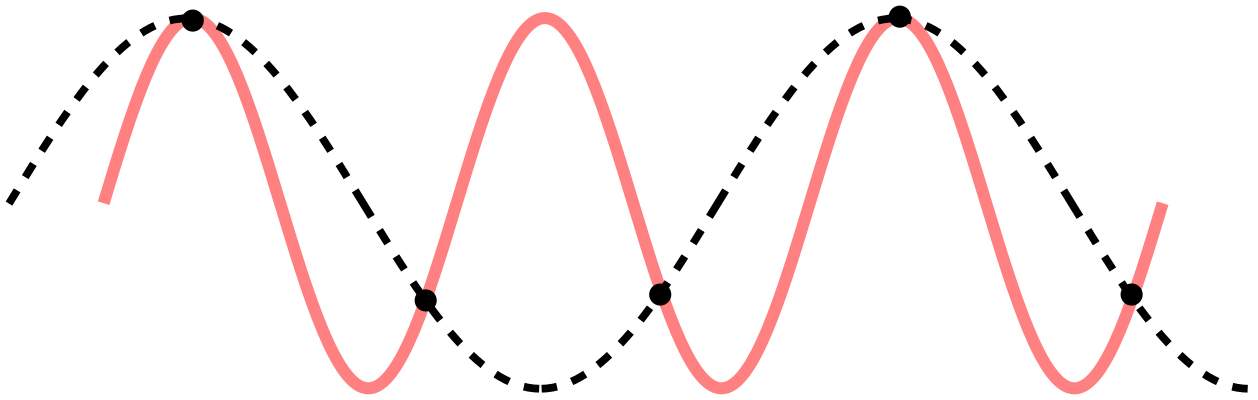
\includegraphics[width=0.8\linewidth]{CPT-sound-nyquist-thereom-1_5percycle.png}
    \end{center}
\end{frame}

\begin{frame}
    \frametitle{Counters}

    \begin{definition}[Monotonic Function]
        A function is called monotonically increasing if for all $x$ and
        $y$ such that $x \leq y$ one has
        $f(x) \leq f(y)$, so $f$
        preserves the order.
    \end{definition}

    \begin{center}
    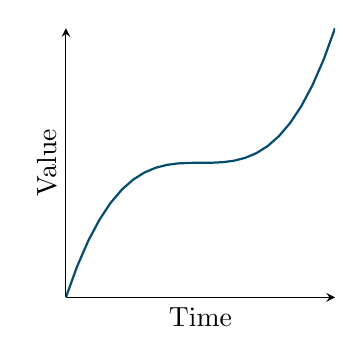
\begin{tikzpicture}[]
        \begin{axis}[
            width=5cm,
            height=5cm,
            xlabel=Time,
            ylabel=Value,
            enlargelimits=false,
            ticks=none,
            axis x line=bottom,
            axis y line=left,
        ]
            \addplot+[no marks, thick] {(x^3};
        \end{axis}
    \end{tikzpicture}
    \end{center}
\end{frame}

\begin{frame}
    \frametitle{Options for Metrics of Events and Cardinality}

    \begin{columns}
        \begin{column}{0.3\linewidth}
            StatsD -- Generate Summary Metrics Per Interval
            \begin{itemize}
                \item Count
                \item Sum
                \item Min
                \item Max
                \item Percentiles
            \end{itemize}
        \end{column}
        \begin{column}{0.7\linewidth}
            \begin{center}
            \begin{tikzpicture}
                \begin{axis}[
                    ylabel=Frequency,
                    xlabel=Cummlative Histogram,
                    ybar interval,
                    grid=none,
                    xtick align=inside,
                    x tick label as interval=false,
                    xtick=,% reset from ybar interval
                    %xticklabel={$(\pgfmathprintnumber\tick - \pgfmathprintnumber\nexttick)$},
                ]

                    \addplot+[hist={cumulative,data=x,data max=120,bins=12}]file {rand_hist.dat};
                \end{axis}
            \end{tikzpicture}
            \end{center}
        \end{column}
    \end{columns}
\end{frame}

\begin{frame}
    \frametitle{Data Alignment and Reporting}

    \begin{center}
        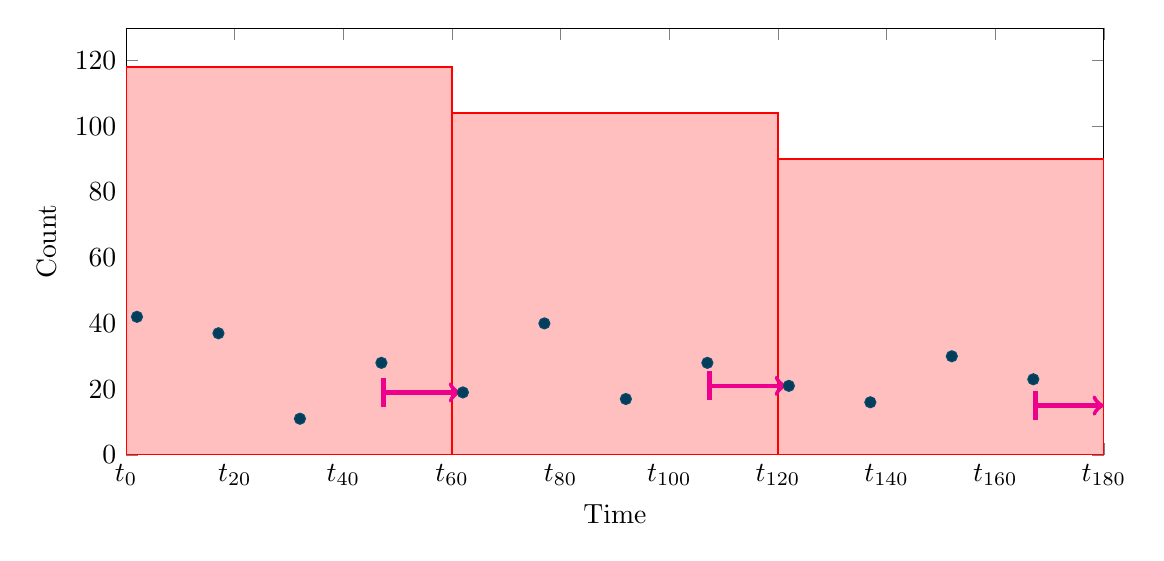
\begin{tikzpicture}[]
            \begin{axis}[
                width=14cm,
                height=7cm,
                xlabel=Time,
                ylabel=Count,
                xticklabel={$t_{\pgfmathprintnumber{\tick}}$},
                xmin=0, ymin=0, xmax=180
            ]
                \addplot+[only marks] coordinates {
                    (2, 42)  % 118
                    (17, 37)
                    (32, 11)
                    (47, 28)
                    (62, 19) % 104
                    (77, 40)
                    (92, 17)
                    (107, 28)
                    (122, 21) % 67+N
                    (137, 16)
                    (152, 30)
                    (167, 23)
                };
                \addplot+[ybar interval,fill=pink,mark=none] coordinates {
                    (0, 118)
                    (60, 104)
                    (120, 90)
                    (180, 0) % ybar interval extra coord
                };
                \draw[ultra thick,magenta,|->,shorten >=1pt] (47,19) to (62,19);
                \draw[ultra thick,magenta,|->,shorten >=1pt] (107,21) to (122,21);
                \draw[ultra thick,magenta,|->] (167,15) to (180,15);
            \end{axis}
        \end{tikzpicture}
    \end{center}
\end{frame}

\begin{frame}[fragile]
    \frametitle{What's an Event?}
Standard apache access log:
\begin{lstlisting}
192.168.1.100 - bdezendorf [12/Sep/2019:31:32:000 -0000] "GET / HTTP/1.0" 200 2216
\end{lstlisting}

JSONLines formatted example of the same event:
\begin{lstlisting}
{
  "timestamp":"2019-09-12T19:31:32.000Z",
  "http_size_bytes": 2216,
  "http_status_code": 200,
  "request": "GET / HTTP/1.0",
  "remote_address": "192.168.1.100",
  "remote_user": "bdezendorf"
}
\end{lstlisting}
\end{frame}

\begin{frame}[fragile]
    \frametitle{Event Schema and Structure}

    \begin{center}
        Lucene isn't just for text anymore!
    \end{center}

    \begin{columns}
        \begin{column}{0.5\textwidth}
    \begin{lstlisting}
{
  "timestamp":"2019-09-12T19:31:32.000Z",
  "http_size_bytes": 2216,
  "http_status_code": 200,
  "request": "GET / HTTP/1.0",
  "remote_address": "192.168.1.100",
  "remote_user": "bdezendorf"
}
    \end{lstlisting}
        \end{column}

        \begin{column}{0.5\textwidth}
            \begin{itemize}
                \item Datetime
                \item IP Addresses
                \item Keyword
                \item Geopoint
            \end{itemize}
        \end{column}
    \end{columns}
\end{frame}

\begin{frame}
    \frametitle{How Do Events Compare to Metrics?}

    Disadvantages

    \begin{itemize}
        \item Events are roughly 100x more expensive than metrics
        \item Costs split evenly in memory, disk, CPU, and network I/O
        \item Guidelines for organization of data is hand wavy at best
    \end{itemize}

    Advantages

    \begin{itemize}
      \item Allows for ex post facto data exploration
      \item Finds needles in haystacks that p99 values can't
    \end{itemize}
\end{frame}

\begin{frame}
    \frametitle{Guidelines for Using Metrics}

    \begin{itemize}
        \item Count Performance
        \item Key Health Indicators
        \item Limited Debugging with Feature Flags
        \item Make a Plan for Cardinality
        \item Look for Histogram Support
        \item Have a ``kit'' for SOA Metrics
        \item Team or Application Namespaces
        \item Identify Important Aggregations and Ditch the Rest
    \end{itemize}
\end{frame}

\begin{frame}
    \frametitle{Guidelines for Using Logs and Events}
    \begin{itemize}
        \item Event size influences speed at every stage of the pipeline
        \item Do as little log processing as possible
        \item Sampling, rollup, and reporting
    \end{itemize}
\end{frame}

\begin{frame}[fragile]
    \frametitle{Use Hashing for Event Management}

    Generate request uuid at the loadbalancer
    \begin{lstlisting}
request_id:19CADF41-11BE-421D-89FA-52DBA8315A1A
    \end{lstlisting}

    MURMUR3 the id, divide by maxint
    \begin{lstlisting}
request_id_sampling_score:0.01799897874
    \end{lstlisting}

    \begin{lstlisting}
if ( [logstash][sampling_score] >= [logstash][long_tail_rate] ){
  mutate {
    replace => [ "[@metadata][retention]", "365" ]
  }
  ruby {
    code => "event.set('[logstash][scaledCount]',
    1 / ( 1 - event.get('[logstash][long_tail_rate]') ))"
  }
}
\end{lstlisting}
\end{frame}

\begin{frame}
    \frametitle{save sampling rate to re-hyrdrate data with later}
    \begin{center}
        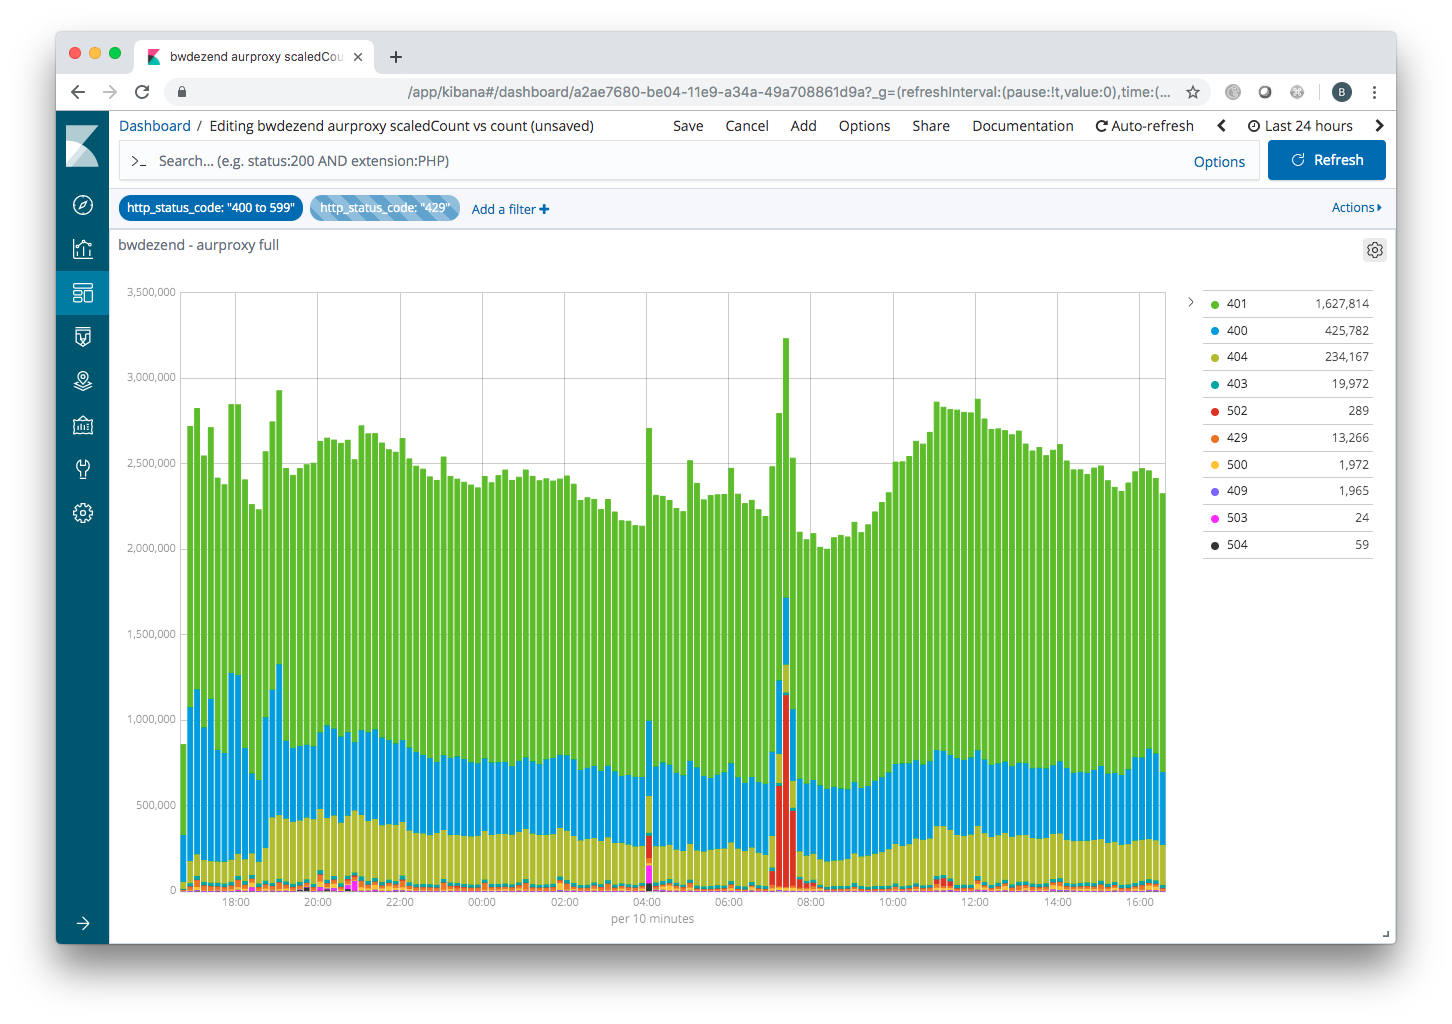
\includegraphics[width=0.8\linewidth]{query-full.png}
    \end{center}
\end{frame}

\begin{frame}
    \frametitle{save sampling rate to re-hyrdrate data with later}
    \begin{center}
        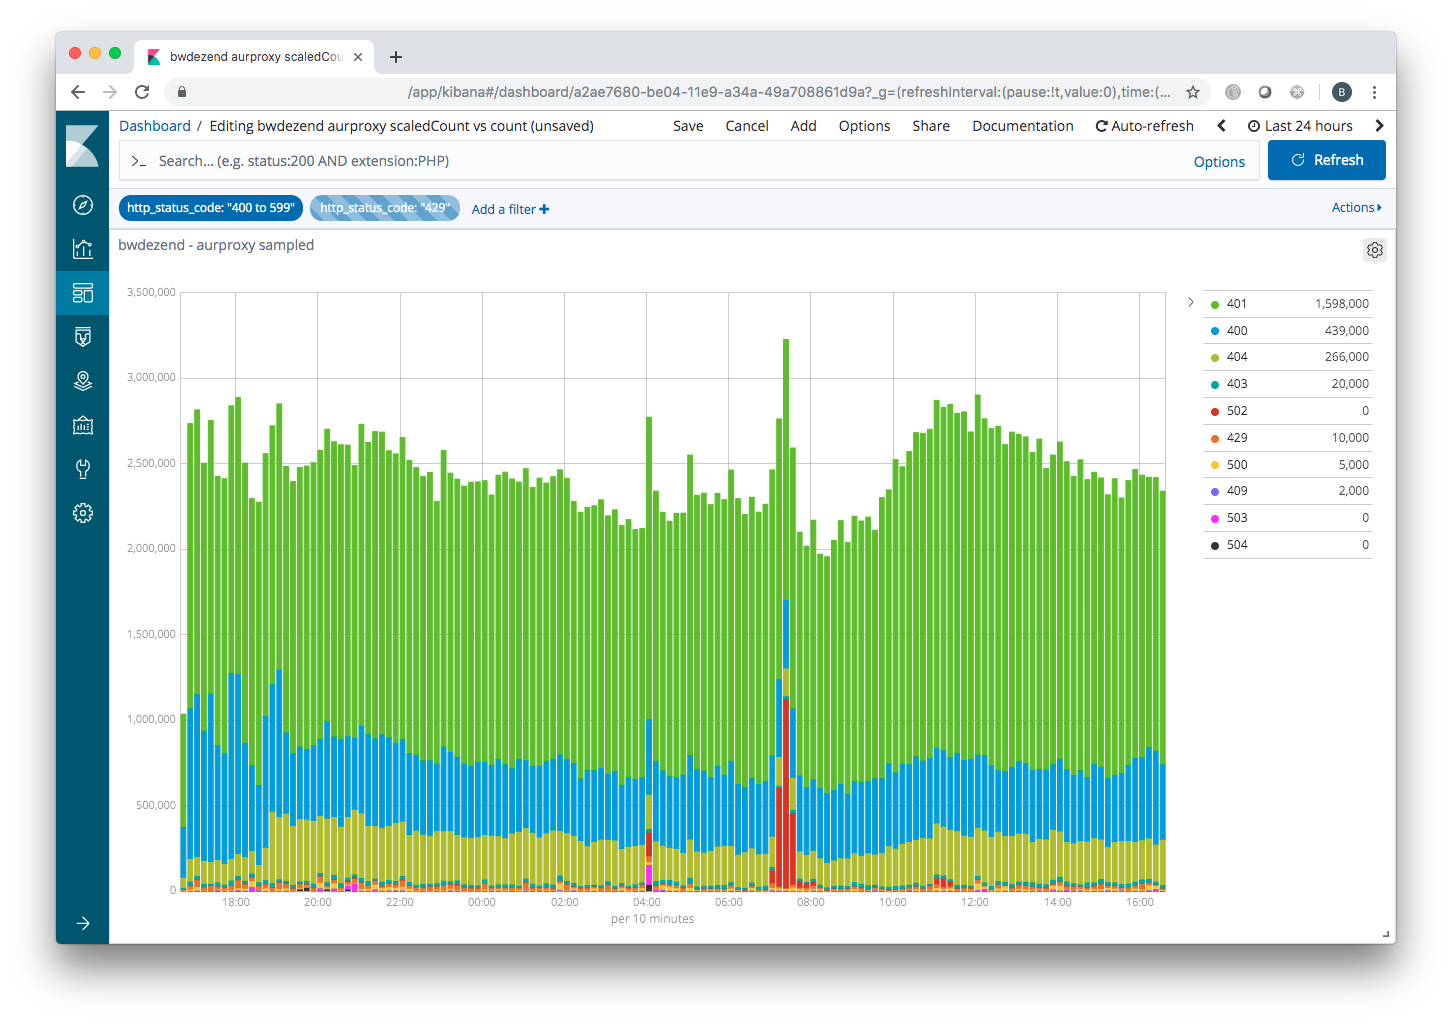
\includegraphics[width=0.8\linewidth]{query-sampled.png}
    \end{center}
\end{frame}

\begin{frame}[standout]
    \begin{center}
        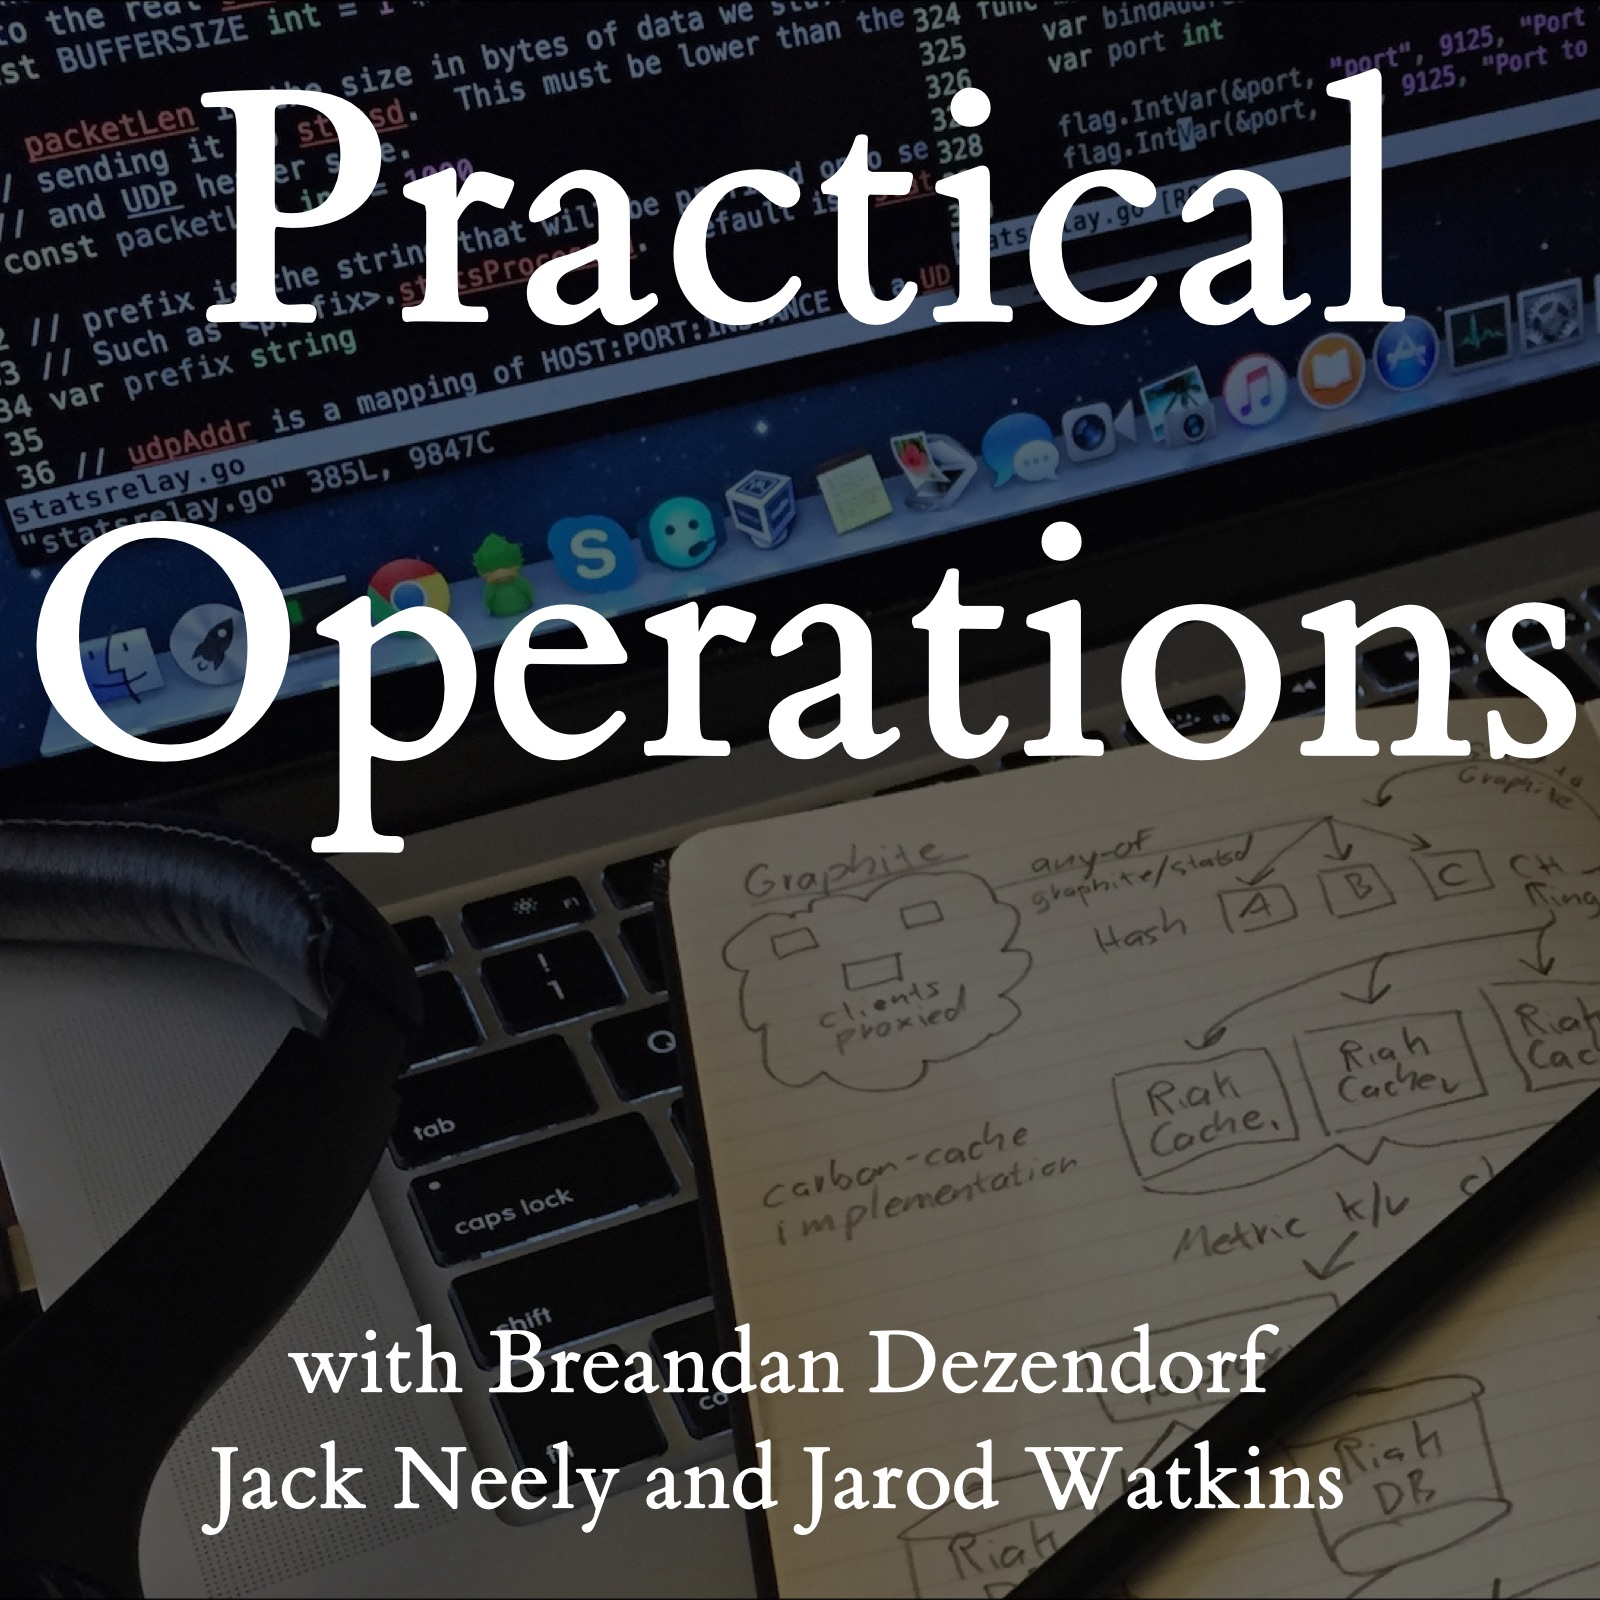
\includegraphics[width=0.5\linewidth]{cover-square.jpg}

        \href{https://operations.fm}{operations.fm}
    \end{center}
\end{frame}

\begin{frame}[standout]
    Thank You!
\end{frame}

\appendix

\begin{frame}[fragile]
    \frametitle{Anomaly Detection Prometheus Examples}

\begin{lstlisting}
  - record: job:http_requests:rate5m
    expr: sum(rate(http_requests_total[5m]))

  - record: job:http_requests:rate5m_forecast
    expr: quantile_over_time(0.5, job:http_requests:rate5m[1h] offset 1h)

  - alert: AnomalyFound
    expr: abs(job:http_requests:rate5m - job:http_requests:rate5m_forecast)
      / job:http_requests:rate5m_forecast > 0.1
    for: 3m
    labels:
      severity: page
    annotations:
      summary: Anomaly Found
      description: Red Alert
      runbook: http://wiki.example.com/AnomalyFound
\end{lstlisting}
\end{frame}

\end{document}
